\documentclass[10pt,a4paper,twoside]{article}
\usepackage[utf8]{inputenc}
\usepackage[francais]{babel}
\usepackage[T1]{fontenc}
    \usepackage[bitstream-charter]{mathdesign}
\usepackage[T1]{fontenc}
\usepackage{amsmath}
\usepackage{amsfonts}
\usepackage{amssymb}
\usepackage{graphicx}
\usepackage{lipsum}
\usepackage[left=2cm,right=2cm,top=2cm,bottom=2cm]{geometry}
\author{Ludovic}
\title{\LaTeX \& Python pour de belles figures}
\begin{document}
\maketitle

\lipsum[1-4]
\begin{figure}[htb]
\begin{center}
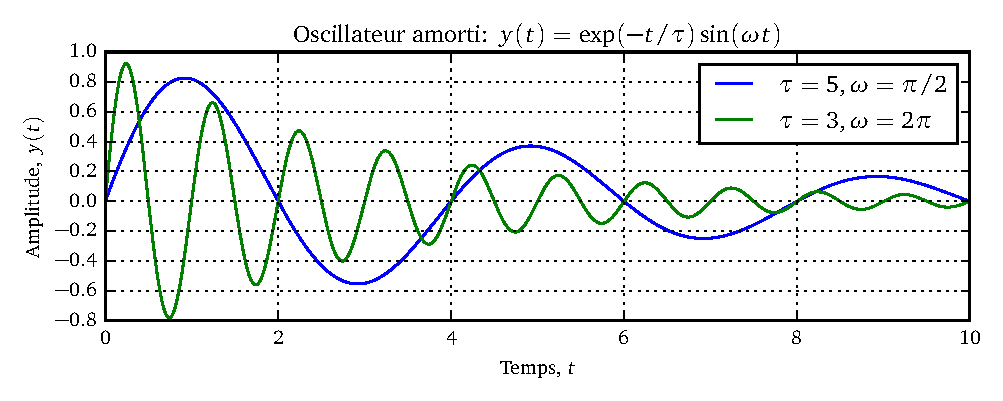
\includegraphics{oscillateur}
\end{center}
\end{figure}
\lipsum[1-4]
\begin{figure}[htb]
\begin{center}
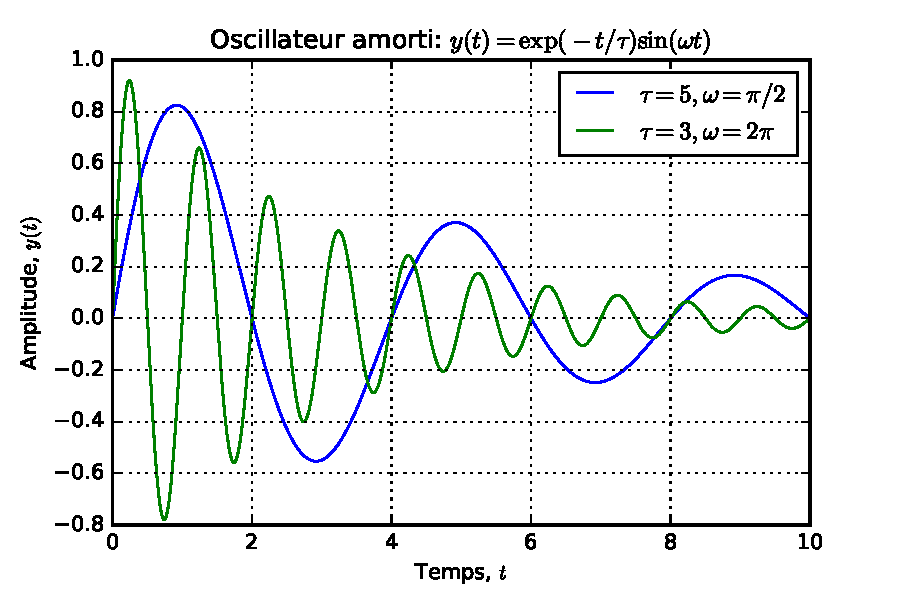
\includegraphics[width = .8\textwidth]{../cachette/oscillateur}
\end{center}
\caption{Elle est cachée\ldots}
\end{figure}
\lipsum[1-8]
\end{document}